\section{Introduction}

\section{Theory}

\subsection{Overview}
\label{sec:Overview}
A comprehensive treatment of the original method, including proofs, can be found in \textit{SSS}.  Here we develop the method specifically for the general linear model (GLM) and describe our own enhancements to the method. While the method can be performed for subject-level inference, we will motivate the method in the context of a group-level analysis, describing how the method can be applied to subject-level \%BOLD estimate maps in order to obtain group-level CSs making confidence statements about \%BOLD effect sizes relating to the entire population from which the participants were drawn.

For a compact domain $S \subset \mathbb{R}^{D}$, e.g.~$D=3$, consider the GLM at location $\bm{s} \in S$,
\begin{equation}
\label{eq:CI_GLM}
\bm{Y}(\bm{s}) = \bm{X}\bm{\beta}(\bm{s}) + \bm{\epsilon}(\bm{s})	
\end{equation}
where $\bm{Y}(\bm{s})$ is an $N \times 1$ vector of observations at  $\bm{s}$, $\bm{X}$ is an $N \times p$ design matrix, $\bm{\beta}(\bm{s})$ is an $p \times 1$ vector of unknown coefficients, and $\bm{\epsilon}(\bm{s})$ an $N \times 1$ vector of mean-zero errors, independent over observations, and with each $\epsilon_i$ having common variance $\sigma^2(\bm{s})$ and some unspecified spatial correlation. (Throughout we use boldface to indicate a vector- or matrix-valued variable.) In the context of a  task-fMRI analysis, $\bm{Y}(\bm{s})$ is a vector of subject-level \%BOLD response estimate maps obtained by applying a first-level GLM to each of the $N$ participants functional data. 

For a $p \times 1$ contrast vector $\bm{w}$, we seek to infer regions of the brain where a contrast of interest $\bm{w}^{T}\bm{\beta}$ has exceeded a fixed threshold  $c$. Particularly, we are interested in the noise-free, population cluster defined as: 
\begin{equation}
\label{eq:CI_excursion}
\Ac = \{\bm{s} \in S : \bm{w}^{T}\bm{\beta}(\bm{s}) \geq c \}.
\end{equation}

Since we are unable to determine this excursion set in practice, our solution is to find spatial CSs: an upper set $\Ahatcp$ and lower set $\Ahatcm$ that surround $\Ac$ for a desired confidence level of, for example, 95\%. We emphasize that these clusters regard the raw units of the signal. Going forward, we assume that the design matrix $\bm{X}$ and contrast $\bm{w}$ have been carefully chosen so that $\bm{w}^{T}\hat{\bm{\beta}}$ has the interpretation of mean \%BOLD change across the group. For example, in a one-sample group fMRI model where data $\bm{Y}$ have \%BOLD units, choosing $\bm{X}$ as a column of 1's and $\bm{w}=(1)$ would ensure that $\bm{w}^{T}\hat{\bm{\beta}}$ has units of \%BOLD change\footnote{For examples of how to set up more complex designs and contrasts, see Figure A.2. in the Appendix A section of \citep{Poldrack2011-bw}.}. In this setting, we wish to obtain an upper CS, $\Ahatcp$, such that we have 95\% confidence all voxels \textit{contained} in this set have a population raw effect size \textit{greater} than, for example, c = 2.0\% BOLD change, and a lower CS, $\Ahatcm$, such that we have 95\% confidence all voxels \textit{outside} of this set have a population raw effect size \textit{less} than 2.0\% BOLD change. Moreover, we desire that the 95\% confidence statement holds simultaneously across both CSs at once.
\textit{SSS} show that a construction of such CSs is possible within the general linear model framework using the following key result. 

\newtheorem{theorem}{Result}
\begin{theorem}
\label{thm:SSS_result}
Consider the general linear model set-up described in (\ref{eq:CI_GLM}). Let $\hat{\bm{\beta}}$ denote the ordinary least squares estimator of $\bm{\beta}$, $\hat{\bm{\beta}}(\bm{s})=(\bm{X}^T\bm{X})^{-1}\bm{X}^T\bm{Y}(\bm{s})$, and define
$v^{2}_{w}=\bm{w}^T(\bm{X}^T\bm{X})^{-1}\bm{w}$ 
%$v^{2}_{w}(\bm{s})=\mathrm{Var}(\bm{w}^T\hat{\bm{\beta}}(\bm{s}))/\sigma^{2}(\bm{s})$ 
to be the normalised variance of the contrast estimate.

Then for a constant $k$, and for upper and lower CSs defined as
$$\Ahatcp := \Bigg\{\bm{s} : \bm{w}^{T}\bm{\hat{\beta}}(\bm{s}) \geq c + k\, \hat{\sigma}(\bm{s}) v_{w} \Bigg\}, \quad \Ahatcm := \Bigg\{\bm{s} : \bm{w}^{T}\bm{\hat{\beta}}(\bm{s}) \geq c - k \,\hat{\sigma}(\bm{s}) v_{w}  \Bigg\},$$ 
the limiting coverage of the CSs is
$$\lim_{n\rightarrow\infty} P  \Bigg[\Ahatcp \subset \Ac \subset \Ahatcm\Bigg] = P \Bigg[\sup_{\bm{s}\in\dAc}|G(\bm{s})|\leq k\Bigg],$$
where $\dAc$ denotes the boundary of $\Ac$, and $G$ is a smooth Gaussian field on $S$ with mean zero, unit variance, and with the same spatial correlation as each $\epsilon_i$. 
\end{theorem}
Result \ref{thm:SSS_result} is subject to continuity of the relevant fields and some basic conditions on the increments and moments of the error field $\bm{\epsilon}$. A list of these assumptions, as well as a proof of Result \ref{thm:SSS_result}, are itemized in \textit{SSS}. 


\begin{figure}[htbp]
\hspace*{-1.5cm}
\label{fig:one_d_intuiton}%
\centering
    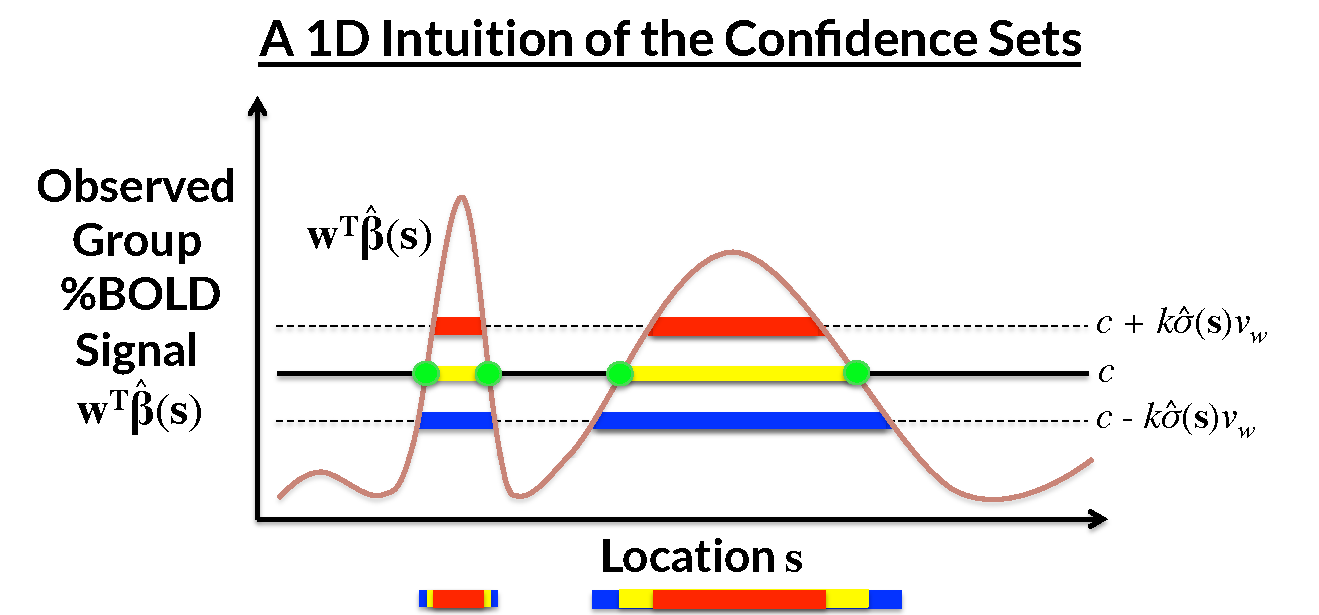
\includegraphics[height=3in]{CIB_One_D_intuition_dot.pdf}
\caption{A demonstration of how the CSs are computed for a realization of the GLM $\bm{Y}(\bm{s}) = \bm{X}\bm{\beta}(\bm{s}) + \bm{\epsilon}(\bm{s})$ in 1 dimension, for each location $\bm{s}$.
The yellow voxels $\Ahatc$ are obtained by thresholding the observed group contrast map at threshold $c$; this is the best guess of $\Ac$, the set of voxels whose true, noise-free raw effect surpasses $c$. 
The red upper CS $\Ahatcp$ and blue lower CS $\Ahatcm$ are computed by thresholding the signal at  $c + k\, \hat{\sigma}(\bm{s}) v_{w}$ and $c - k\, \hat{\sigma}(\bm{s}) v_{w}$, respectively. 
We have $(1-\alpha)100\%$ confidence that $\Ahatcp \subset \Ac \subset \Ahatcm$, i.e.~that $\Ahatcp$ (red) is completely within the true $\Ac$, and $\Ac$ is completely within $\Ahatcp$ (blue). 
We find the critical value $k$ from the $(1-\alpha)100$ percentile of the maximum distribution of the absolute error process over the estimated boundary $\dAhatc$ (green \newmoon's) using the Wild $t$-Bootstrap; $\hat\sigma$ is the estimated standard deviation and $v_w$ is the normalised contrast variance.}
\end{figure}

For a pre-determined confidence level $1 - \alpha$ (e.g. $1 - \alpha = 95\%$),  by choosing $k$ such that 
\begin{equation}
\label{eq:probability_statement}
P \Bigg[\sup_{\bm{s}\in\dAc}|G(\bm{s})|\leq k\Bigg] \geq 1-\alpha,
\end{equation}
Result \ref{thm:SSS_result} ensures with asymptotic probability of $1 - \alpha$ that $\Ahatcm$ contains the true  $\Ac$,  and $\Ahatcp$ is contained within $\Ac$. In practice,  $k$ is determined as the $(1-\alpha)100$ percentile of the maximum distribution of the asymptotic absolute error process $|G(\bm{s})|$ over the true boundary set $\dAc = \{\bm{s} : \bm{w}^{T}\bm{\beta}(\bm{s}) = c\}.$ The upper CS taken away from the lower CS $\Big(\Ahatcm \ \cap \ \big(\Ahatcp\big)^{\mathsf{c}}\Big)$ can be interpreted analogously to a standard confidence interval: with a confidence of $1 - \alpha$, we can assert the true boundary $\dAc$ lies within this region. Here, we allude to the classical frequentist interpretation of confidence, where stated precisely, there is a probability of $1 - \alpha$ that the region $\Big(\Ahatcm \ \cap \ \big(\Ahatcp\big)^{\mathsf{c}}\Big)$ computed from a future experiment fully encompasses the true set boundary $\dAc$.

Application of Result \ref{thm:SSS_result} presents us with two challenges: that the boundary set $\dAc$ and the critical value $k$ are both unknown.  To solve the first problem, \textit{SSS} propose using $\dAhatc$ as a plug-in estimate of $\dAc$. There remain, however, technicalities at to how the boundary is determined in any non-abstract setting, and in particular in a 3D image. In Section \ref{sec:boundary_discrete_lattice} we propose our own novel method for boundary estimation. Before that, we address the second problem, finding the critical value \textit{k} via a Wild Bootstrap resampling scheme. 

\subsection{The Wild Bootstrap Method for Computation of \textit{k}}
\label{sec:wild_bootstrap}
To apply Result \ref{thm:SSS_result}, we require knowledge of the tail distribution of the limiting Gaussian field $G$ along the boundary $\dAc$. However, the distribution of this field is unknown, because it is dependent on the unknown spatial correlation of the errors $\epsilon_i$. We can approximate the maximum distribution of $G$ using the Gaussian Wild Bootstrap \citep{Chernozhukov2013-wz}, also known as the Gaussian Multiplier Bootstrap, which multiplies residuals by random values to create surrogate instances of the random errors.

\textit{SSS} construct $G$ as follows: The standardized residuals,
\begin{equation}
\label{eq:SSS_standardized_residuals}
\tilde{\bm{\epsilon}}(\bm{s}) = \frac{ \bm{Y}(\bm{s}) - \bm{X}\hat{\bm{\beta}}(\bm{s})}{\sigma(\bm{s})},
\end{equation}
%
are  multiplied by i.i.d.~Gaussian random variables, $r^*_1,...,r^*_N$,  summed and scaled,
\begin{equation}
\label{eq:SSS_residual_field}
G^*(\bm{s}) = \frac{1}{\sqrt{N}}\sum_{i=1}^{N} r^*_i\tilde{\epsilon}_{i}(\bm{s}),
\end{equation}
producing a field $G^*$ with approximately the same covariance as each error $\epsilon_i$, where the superscript asterisk ($*$) indicates these are just one of many bootstrap realizations. With $B$ bootstrap samples $G^*$, we choose $k$ as the $(1 - \alpha)100$ percentile of the $B$ suprema   $\sup_{\bm{s}\in\dAhatc}|G^*(\bm{s})|$ to approximate the LHS of (\ref{eq:probability_statement}) and apply Result \ref{thm:SSS_result} to obtain the CSs. 

Up to this point, we have summarized the Gaussian Wild Bootstrap methodology as proposed in \textit{SSS}. However, when applying this method to our own simulations, we consistently found that our coverage results fell below the nominal level.  This was particularly severe for 3D simulations we conducted using a small sample size (N = 60), where our results in some cases suffered from under-coverage 40\% or more below the nominal level (see \textbf{REFERENCE COMPARISON FIGURE}). Hence we made two alterations: First, while \textit{SSS} used Gaussian multipliers, we found improved performance using Rademacher variables, where each $r_i$ takes on 1 or -1 with  probability 1/2; others have also reported improved performance with Rademacher variables as well \citep{Davidson2008-qh}. Second, we implemented a Wild $t$-Bootstrap \citep{Telschow2019-lg} method, normalizing the bootstrapped residuals $\tilde{\epsilon}_{i}(\bm{s})$ by their standard deviation $\hat{\sigma}^*$. This detail was omitted in the proof of Result 1 provided in \textit{SSS}, where the true standard deviation was assumed to be known. By taking into account the estimation of the standard deviation via the Wild $t$-Bootstrap, we found improved performance for moderate sample sizes. The Wild $t$-Bootstrap version of $G$ is
\begin{equation}
\label{eq:wild_bootstrap_G}
\tilde{G}^{*}(\bm{s}) = \frac{1}{\sqrt{N}}\sum_{i=1}^{N} r^*_i\frac{\tilde{\epsilon}_{i}(\bm{s})}{\hat{\sigma}^*(\bm{s})},
\end{equation}
 where $\hat{\sigma}^{*}(\bm{s})$ is the standard deviation of the present realization of the bootstrapped residuals $r^*_i\tilde{\epsilon}_{i}(\bm{s})$. We then determine $k$ as described above but using $\tilde{G}^{*}$ instead of $G^*$. Going forward, we refer to this method as the ``Wild $t$-Bootstrap", to be contrasted with the original ``Gaussian Wild Bootstrap" method proposed in \textit{SSS}.

With these two alterations we found a dramatic increase in performance for small sample sizes in 3D simulations. 
Notably, in contrast to the Gaussian Wild Bootstrap, our simulation results presented in Section \ref{sec:Results} suggest that empirical coverage rates for this modified procedure remain valid, i.e.~stay \textit{above} the nominal level.  

\subsection{Approximating the Boundary on a Discrete Lattice}
\label{sec:boundary_discrete_lattice}

In the previous section, we described the ideal bootstrap procedure used to obtain the maximum distribution of $G$ along the boundary $\dAc$ in order to apply Result \ref{thm:SSS_result}. However, in any practical application, data will be observed on a discrete grid of lattice points at a fixed resolution. Therefore, a key challenge is how to appropriately approximate the true continuous boundary $\dAc$ from the lattice representation of the data. 

In \textit{SSS}, spline-interpolation was used to estimate a 1D boundary at a resolution greater than their 2D sampled field (\textit{SSS}, Section 4.1). However, to apply the method to fMRI data we will work with 3D images, and estimating a 2D spline boundary for a 3D field is more involved, requiring careful tuning of the spline basis to accommodate the structure of the 3D signal. Instead, we choose to use a first-order weighted linear interpolation method to approximate the signal values at estimated locations along the true, continuous boundary $\dAc$, providing a method of boundary estimation that is less computationally intensive than spline interpolation.

Consider two adjacent points on the lattice, $\bm{s_O}$ and $\bm{s_I}$, such that $\bm{s_O}$ lies outside of $\Ac$, while $\bm{s_I}$ lies inside $\Ac$. By the definition of $\Ac$, $\bm{w}^{T}\bm{\beta}(\bm{s_O}) < c$, and $\bm{w}^{T}\bm{\beta}(\bm{s_I}) \geq c$. Under the assumption that the component of the signal between $\bm{s_O}$ and $\bm{s_I}$ increases linearly, we can find the location $\bm{s}^{*}$ between $\bm{s_O}$ and $\bm{s_I}$ such that $\bm{w}^{T}\bm{\beta}(\bm{s}^{*}) = c$, our estimate of where the true continuous boundary $\dAc$ crosses between $\bm{s_O}$ and $\bm{s_I}$. We can then construct a linear interpolant for the location $\bm{s}^{*}$, using weights
\begin{equation}
\label{eq:interpolation_weights}
m_{1} = \frac{\bm{w}^{T}\bm{\beta}(\bm{s_I}) - c}{\bm{w}^{T}\bm{\beta}(\bm{s_I}) - \bm{w}^{T}\bm{\beta}(\bm{s_O})}, \quad m_{2} = \frac{c - \bm{w}^{T}\bm{\beta}(\bm{s_O})}{\bm{w}^{T}\bm{\beta}(\bm{s_I}) - \bm{w}^{T}\bm{\beta}(\bm{s_O})},
\end{equation}
for locations $\bm{s_O}$ and $\bm{s_I}$, respectively. By construction, applying $m_1$ and $m_2$ to the contrast image returns the threshold: $m_1 \bm{w}^{T}\bm{\beta}(\bm{s_O}) + m_2 \bm{w}^{T}\bm{\beta}(\bm{s_I}) = \bm{w}^{T}\bm{\beta}(\bm{s}^{*}) = c$. Applied to standardized residuals %(\ref{eq:6}),
$\tilde{\bm{\epsilon}}(\bm{s_O})$ and $\tilde{\bm{\epsilon}}(\bm{s_I})$, we can likewise obtain the residuals at the estimated continuous boundary point $\tilde{\bm{\epsilon}}(\bm{s}^{*}) = m_1 \tilde{\bm{\epsilon}}(\bm{s_O}) + m_2\tilde{\bm{\epsilon}}(\bm{s_I})$.

By repeating this procedure for all adjacent points $\bm{s_O}$ and $\bm{s_I}$ that lie on the lattice  either side of $\dAc$, we are able to estimate the standardized residual values at locations that should approximately sample the true continuous boundary $\dAc$, and thus we can apply the ideal bootstrap procedure outlined in Section \ref{sec:wild_bootstrap}. Of course, in practice we apply this interpolation method on the observed, noisy data, using the plug-in estimated boundary $\dAhatc$. 

In the simulation results in Section \ref{sec:Results}, we assess performance of the method when the bootstrap procedure is carried out over the true boundary $\dAc$, and the plug-in estimated boundary $\dAhatc$ that must be used in practice. 

\subsection{Assessment of Continuous Coverage on a Discrete Lattice}
\label{sec:coverage_assessment}

\begin{figure}[h!!]\label{fig:highres_lowres}%
\centering
\subfigure[Low Resolution Simulation]{\label{fig:lowres}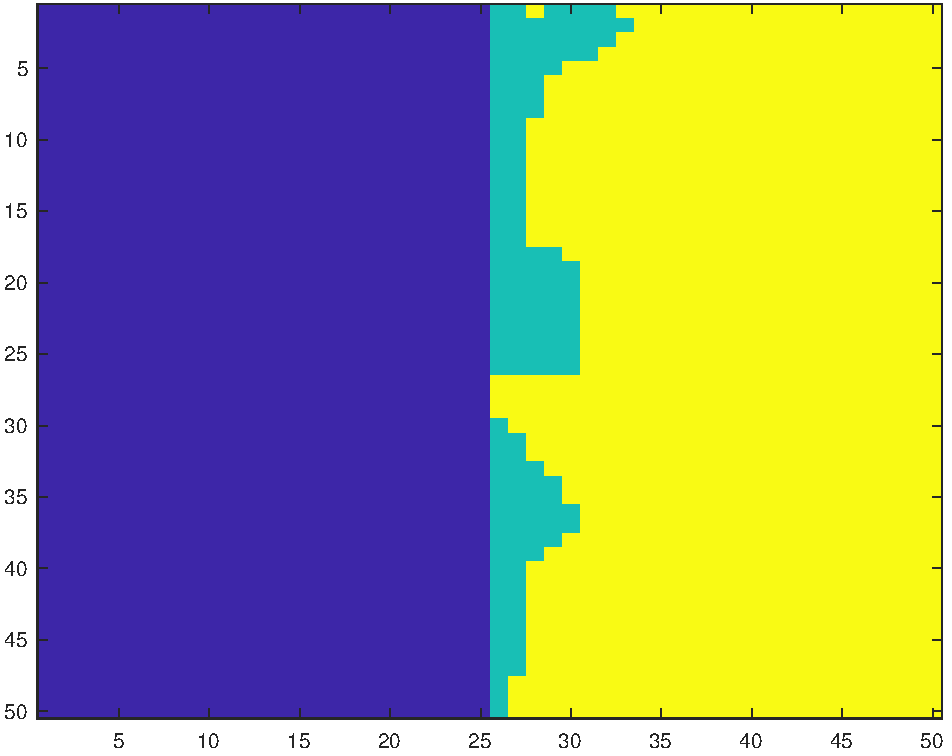
\includegraphics[height=2in]{CIB_low_res_example.pdf}}
\subfigure[High Resolution Simulation]{\label{fig:highres}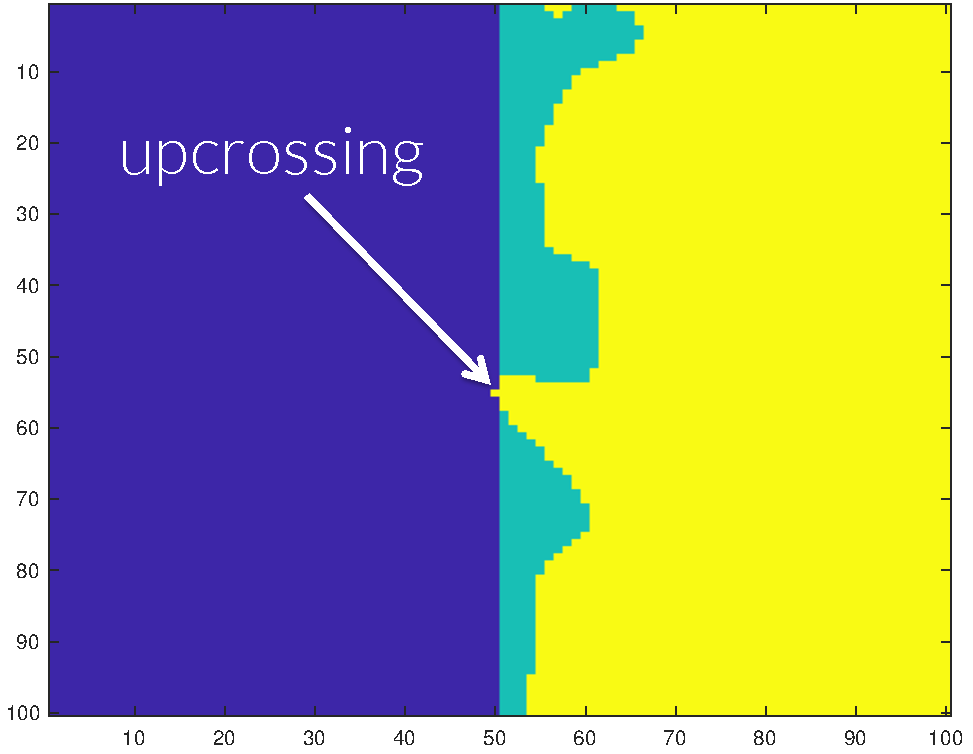
\includegraphics[height=2in]{CIB_high_res_example.pdf}}
\caption{Demonstrating the resolution issue for testing the subset condition $\Ahatcp \subset \Ac \ \subset \Ahatcm$. \\ \textbf{Figure \ref{fig:lowres}:} Here $\Ac$ is comprised of the right half of the image (all green and yellow pixels), and $\Ahatcp$ is shown as yellow pixels. It appears that $\Ahatcp \subset \Ac$. \\ \textbf{Figure \ref{fig:highres}:} The same configuration as \textbf{Fig. \ref{fig:lowres}} at double the resolution. Here, we have enough detail to see that $\Ahatcp$ has crossed the boundary $\dAc$ (yellow seeping into blue), and the subset condition $\Ahatcp \subset \Ac$ has been violated.}
\end{figure}

In testing the finite-sample validity of our method through simulation, it is imperative that we are able to accurately measure when violations of the subset condition $\Ahatcp \subset \Ac \subset \Ahatcm$ occur. 
While this may seem a trivial task, as touched on in the previous section, the boundaries of each of these three sets can become ambiguous when data are collected on a discrete lattice. 

To illustrate this point, consider the configuration of sets displayed in Fig. \ref{fig:lowres}. In this instance, suppose the right half of the image corresponds to $\Ac$ (green pixels overlapped by yellow), and yellow pixels belong to $\Ahatcp$. We wish to determine whether the condition $\Ahatcp \subset \Ac$ has been violated or not. One may argue that at the resolution for which the data have been acquired, all pixels that belong to $\Ahatcp$ also belong to $\Ac$, and therefore no violation has  occurred. However, the example presented in Fig. \ref{fig:lowres} has in fact been derived from a 2D simulation conducted at a higher resolution: this $50 \times 50$ simulation was obtained by down-sampling a $100 \times 100$ grid by dropping every other pixel. 
Fig. \ref{fig:lowres} displays the sets $\Ac$ and $\Ahatcp$ from the down-sampled, low resolution simulation, while Fig. \ref{fig:highres} shows the same set of results at the original resolution. In Fig. \ref{fig:highres} we see that there \textit{has} been an upcrossing of the yellow pixels belonging to $\Ahatcp$ over the boundary of the green, and therefore the subset condition $\Ahatcp \subset \Ac$ \textit{has} been violated. From this simulation, it is clear that when we conclude that no violation has occurred in situations like Fig. \ref{fig:lowres}, our empirical coverage will miss violations and be positively biased. By an analogous argument the same issue occurs when testing violations of $\Ac \subset \Ahatcm$.

In \textit{SSS} this direct comparison of the lattice representation of the three sets was used to assess coverage in the simulations. While  they observed this phenomenon of missed violations leading to over-coverage, the proposed solution was to sequentially increase the resolution of the data. We instead again make use of interpolation.

Since, in simulation, we know the true continuous mean image and $\Ac$, following the method described in Section \ref{sec:boundary_discrete_lattice} we can obtain weights $m_1$ and $m_2$ to interpolate between points $\bm{s_O}$ and $\bm{s_I}$ either side of the true, continuous boundary $\dAc$, in order to find a location $\bm{s^*}$ that approximately lies on the boundary (if the true mean is linear, it would be exactly on the boundary). To determine if $\bm{s^*} \in \Ahatcp$, we then re-apply the weights $m_1$ and $m_2$ and assess whether
\begin{equation}
\label{eq:interpolation_in_action}
\bm{w}^{T}\bm{\hat{\beta}}(\bm{s^{*}}) - k\, \hat{\sigma}(\bm{s^{*}}) v_{w} = m_1 \Bigg( \bm{w}^{T}\bm{\hat{\beta}}(\bm{s_O}) - k\, \hat{\sigma}(\bm{s_O}) v_{w} \Bigg) + m_2 \Bigg( \bm{w}^{T}\bm{\hat{\beta}}(\bm{s_I}) - k\, \hat{\sigma}(\bm{s_I}) v_{w} \Bigg) \geq c.
\end{equation}
 If the inequality holds, then by definition $\bm{s^{*}} \in \Ahatcp$. Otherwise, $\bm{s^{*}} \notin \Ahatcp$, and therefore we can conclude that the subset condition $\Ahatcp \subset \Ac$ has been violated. By checking whether $\bm{w}^{T}\bm{\hat{\beta}}(\bm{s^{*}}) + k\, \hat{\sigma}(\bm{s^{*}}) v_{w} \geq c$, we can similarly test for a violation of $\Ac \subset \Ahatcm$.
 
By applying this interpolation scheme to all pairs of lattice points with one point inside, one outside, the lattice representation of the boundary, we have devised a method to more accurately assess violations of the subset condition $\Ahatcp \subset \Ac \ \subset \Ahatcm$ for configurations similar to \ref{fig:lowres}. We applied this method for testing the subset condition in our simulations alongside a direct comparison of the lattice representations of the three sets of interest as was done in \textit{SSS}. The addition of the weighted interpolation method caused a considerable decrease in the empirical coverage results towards the nominal level in all of our 3D simulations. Using the direct comparison of the three sets on its own here essentially determined total empirical coverage ($\Ahatcp \subset \Ac \ \subset \Ahatcm$ for all simulation runs), even when using small sample sizes and a low nominal coverage level. This is likely to be because the discrete lattice of observed data points is relatively less dense inside the true continuous process for larger, 3D settings, and therefore more violations of the subset condition are missed if only a direct comparison of the lattice representation of the CSs is carried out.

\section{Method}
 
\subsection{Simulations}

\subsection{Implementation of Contour Inference}

\subsection{2D Simulations}

\subsection{3D Simulations}

\subsection{Application to Human Connectome Project Data}

\section{Results}
\label{sec:Results}

\subsection{2D Simulations}

\subsection{3D Simulations}

\subsection{Human Connectome Project}

\section{Discussion}

\subsection{Limitations}

\section{Conclusion}

\section{Toolbox}